\documentclass[tikz,border=2pt]{standalone}
\usepackage{amsmath,amssymb}
\usepackage{pgfplots}
\pgfplotsset{compat=1.18}
\usetikzlibrary{arrows.meta}
\begin{document}
% Records in an i.i.d. continuous sequence: eight observations, the running maximum as a
% staircase, and the records (new running maxima) at positions 1, 3, 5 and 8.
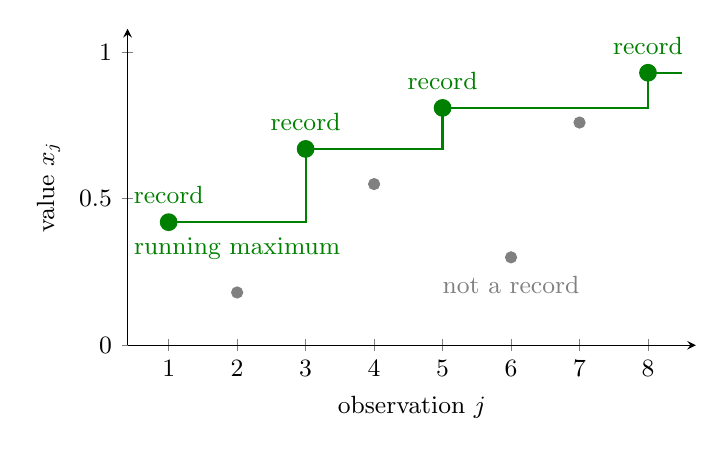
\begin{tikzpicture}[font=\small, >={Latex[length=2mm]}]
  \begin{axis}[
    width=8.8cm, height=5.6cm, axis lines=left,
    xmin=0.4, xmax=8.7, ymin=0, ymax=1.08,
    xtick={1,...,8}, ytick={0,0.5,1},
    xlabel={observation $j$}, ylabel={value $x_j$},
    clip=false
  ]
    % running maximum
    \addplot[green!50!black, thick, const plot]
      coordinates {(1,0.42) (3,0.67) (5,0.81) (8,0.93) (8.5,0.93)};
    % non-records
    \addplot[only marks, mark=*, mark size=2pt, gray]
      coordinates {(2,0.18) (4,0.55) (6,0.30) (7,0.76)};
    % records
    \addplot[only marks, mark=*, mark size=3pt, green!50!black]
      coordinates {(1,0.42) (3,0.67) (5,0.81) (8,0.93)};
    \node[green!50!black, anchor=south] at (axis cs:1,0.45) {record};
    \node[green!50!black, anchor=south] at (axis cs:3,0.70) {record};
    \node[green!50!black, anchor=south] at (axis cs:5,0.84) {record};
    \node[green!50!black, anchor=south] at (axis cs:8,0.96) {record};
    \node[gray, anchor=north] at (axis cs:6,0.27) {not a record};
    \node[green!50!black, anchor=north] at (axis cs:2,0.40) {running maximum};
  \end{axis}
\end{tikzpicture}
\end{document}
